\documentclass[a4paper,10pt]{article} %default
\usepackage{geometry}
\usepackage{fontspec}
\usepackage[normalem]{ulem}
\usepackage{color}
\usepackage{listings}
\usepackage{multicol}
\usepackage{amsmath}
\usepackage{amssymb}
\usepackage{mathtools}
\usepackage{xfrac}
\usepackage{multirow}
\usepackage{abraces}
\geometry{top = 25mm, lmargin=10mm, rmargin=10mm, bottom=10mm}
\pagestyle{empty}
\setlength{\parindent}{0pt}
\setlength{\multicolsep}{0.5em}
\setlength{\columnsep}{0.7cm}


\lstset{
    basicstyle=\ttfamily,
    numberstyle=\ttfamily,
    numbers=left,
    backgroundcolor=\color[rgb]{0.9,0.9,0.9},
    columns=fullflexible,
    keepspaces=true,
    frame=lr,
    framesep=8pt,
    framerule=0pt,
    xleftmargin=20pt,
    xrightmargin=30pt,
    mathescape
}

\newcommand{\specialcell}[2][c]{%
    \begin{tabular}[#1]{@{}l@{}}#2\end{tabular}}
\newcommand{\dimo}[1]{%
    \smallbreak \par \hfill\begin{minipage}{0.92\linewidth}{ \scriptsize {\textbf{\em{Dim.}}} {#1} }\end{minipage} \smallskip \par}
\newcommand{\mdim}[1]{%
    \smallbreak \par \hfill\begin{minipage}{0.95\linewidth}{ \scriptsize {\textbf{\em{Dim.}}} {#1} }\end{minipage} \smallskip \par}
\newcommand{\mtheorem}[1]{%
    {\hspace*{-10pt} \textsc {#1}}}
\newcommand{\malgorithm}[1]{%
    {\bigbreak \par \hspace*{4pt} \underline{\textbf {#1}}}}
\newcommand{\msection}[1]{%
    {\newpage\bigbreak \bigbreak \par \hfil \huge \textsc {#1}}\par}
\renewcommand{\b}[1]{%
    {\textbf{#1}}}
\renewcommand{\t}[1]{%
    {\texttt{#1}}}
\renewcommand{\v}[1]{%
    {\underline{#1}}}
\newcommand{\mdef}[1]{%
    {\smallbreak\par\begin{tabular}{ll} \textbf{Def.$\;\;$} & \begin{minipage}[t]{0.80\columnwidth}\normalsize  {#1}\end{minipage}\tabularnewline \end{tabular}}\smallskip\par}
\newcommand{\ldef}[1]{%
    {\smallbreak\par\normalsize\textbf{\underline{Def.}} {#1} \smallbreak}}
\newcommand{\lprop}[1]{%
    {\smallbreak\par\normalsize\textbf{\underline{Prop.}} {#1} \smallbreak}}
\newcommand{\ltheorem}[1]{%
    {\smallbreak\par\normalsize\textbf{\underline{Th.}} {#1} \smallbreak\par}}
\newcommand{\ldim}[1]{%
    {\smallbreak\par\scriptsize\emph{\textbf{Dimostrazione}} {#1} \par}}
\newcommand{\loss}[1]{%
    {\smallbreak\par\scriptsize\emph{\textbf{Osservazione}} {#1} \par}}
\newcommand{\mcomment}[1]{%
    {\hfill \scriptsize {#1}}}
\newcommand{\mprop}[1]{%
    {\smallbreak\par\begin{tabular}{ll} \textbf{Prop.} & \begin{minipage}[t]{0.8\columnwidth}\emph  {#1}\end{minipage}\tabularnewline \end{tabular}}\smallskip\par}
\newcommand{\shortoverbrace}[2]{\aoverbrace[U]{#1}^{\mathclap{#2}}}%

\makeatletter
\g@addto@macro\normalsize{%
  \setlength{\abovedisplayskip}{3.0pt plus 2.0pt minus 5.0pt}%
  \setlength{\belowdisplayskip}{3.0pt plus 2.0pt minus 5.0pt}%
}
\makeatother




\newcommand{\tsection}[1]{%
    {\center \bigbreak \par \hfil \huge \textsc {#1}} \bigbreak \par}




\usepackage[colorlinks]{hyperref}
\usepackage{graphicx}
\usepackage{caption,subcaption}
\graphicspath{ {images/} }
\usepackage{float}
\usepackage{wrapfig}
\restylefloat{figure}
\begin{document}


\begin{titlepage}
    \centering
    \vbox{}
    \vspace{1.5cm}
    {\scshape\LARGE La Sapienza university of Rome  \par}
    \vspace{2cm}
    {\Huge \bfseries Raymarching vulcanic archipelagos \par}
    \vspace{1cm}
    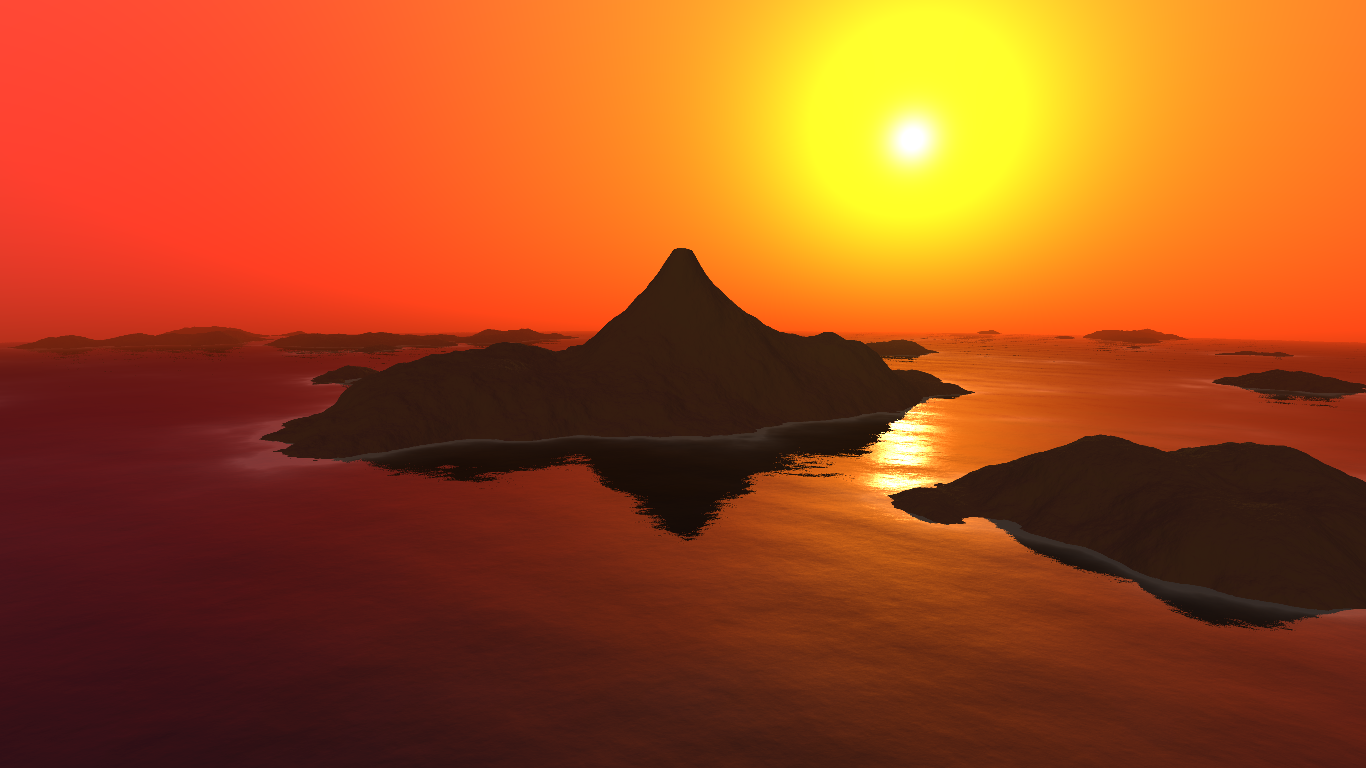
\includegraphics[width=\textwidth, height=12cm]{main2} \par
    Try it live! \url{https://www.shadertoy.com/view/4dcyzM} \par
    %\vspace{2cm} \par
    \vfill \par
    \Large
    \emph{ Luca di Bartolomeo} \par
    \vspace{1cm}
    \textsc{Computer graphics course final project \\ Teaching professor: }  Fabio Pellacini
    \vfill
    \today


\end{titlepage}

\tsection{1. Terrain generation}

%ciao


\begin{wrapfigure}[41]{l}{0.4\textwidth}
    \vspace{-1em}
    \centering
    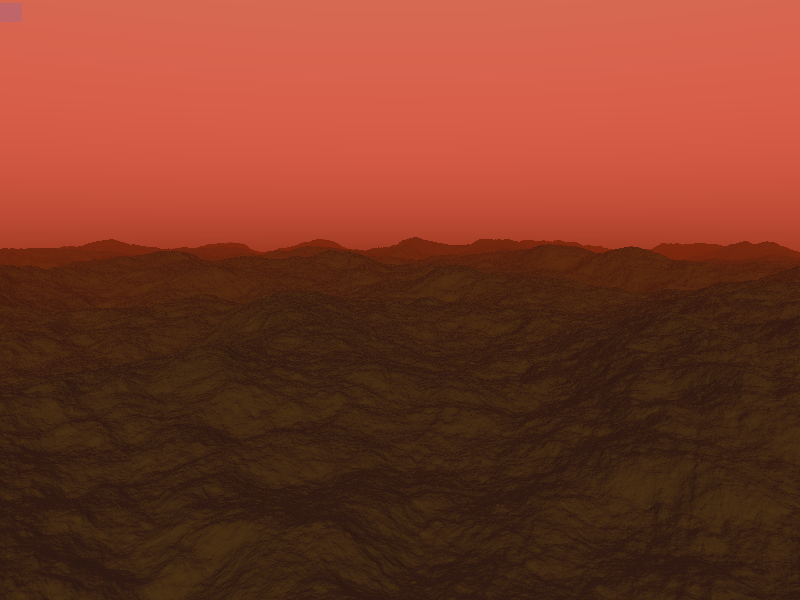
\includegraphics[width=0.38\textwidth]{fbm2} \par
    Figure 1: Normal fbm terrain \par
    \vspace{1em}

    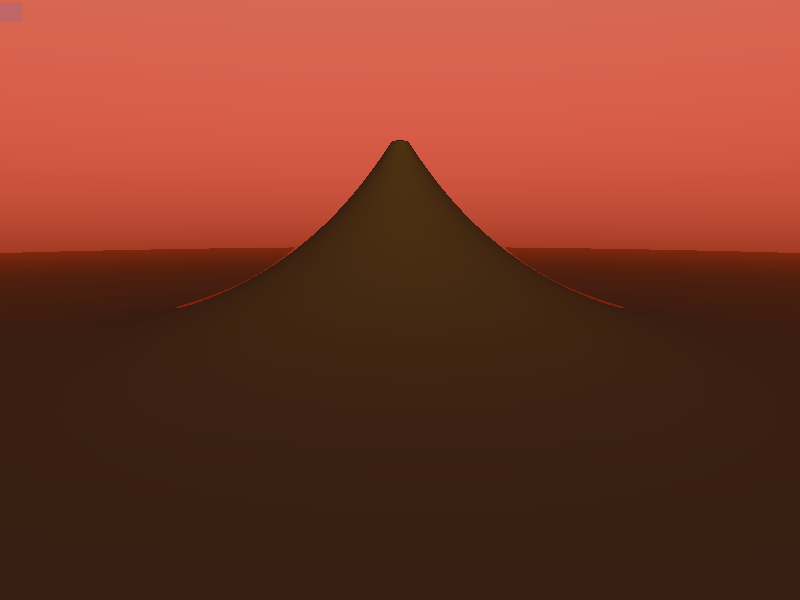
\includegraphics[width=0.38\textwidth]{elevation2} \par
    Figure 2: $e^{-\sqrt{x^2 + z^2}}$ \par
    \vspace{1em}

    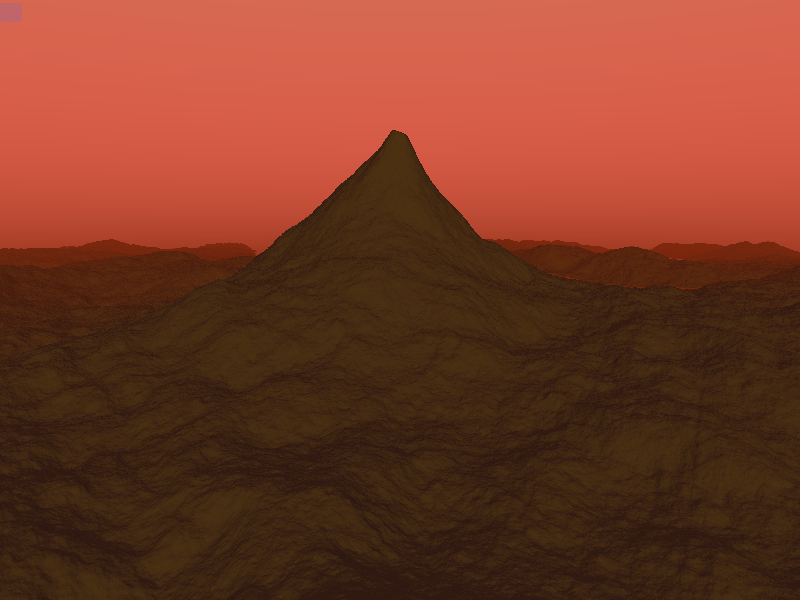
\includegraphics[width=0.38\textwidth]{elevationfbm2} \par
    Figure 3: fbm + $e^{-\sqrt{x^2 + z^2}}$
\end{wrapfigure}

\large
All the terrain is procedurally generated and represented as a heightmap. It is a combination of a noise function and an elevation function.

Initially, the height of the terrain in a particular point is generated through a \b{fractal brownian motion} (fbm) noise, which is defined as:

\[
    fbm(x, z) = \sum_{i=1}^{n} \left(\frac{1}{2}\right)^i \cdot noise(2^i x, 2^i z)
\]


where $n$ is the number of \emph{octaves}. In fact, the $fbm$ function is a sum of the same noise, each time with half the amplitude but twice the 
frequency. The $noise$ function is a normal value noise generator (gradient noise like Perlin can be used too). 

Assuming we know the analytical derivatives
of the $noise$, the derivatives of $fbm$ are the weighted sum of the derivatives of the $noise$ for each octave.
Thanks to this, the normal of the terrain can be calculated using a closed formula, without occurring in the time and precision penalties of numerical
derivation.

The $fbm$ heightmap, with the right parameters,  produces a landscape like in Figure 1; to realize the volcano the heightmap was summed to this 
\b{elevation} function:

\[
   h \cdot e^{-k \sqrt{(x - x_0)^2 + (z - z_0)^2}} 
\]

where $(x_0, z_0)$ are the desired coordinates of the volcano (which for simplicity are $(0,0)$ ), $h$ its height, and $k$ its width. The effect of this function can be seen in Figure 2.

The crater is simply obtained by subtracting:

\[
    \max(0, w - \sqrt{x^2 + z^2})
\]

where $w$ is the width of the crater.

By summing those three, the result is Figure 3: a natural-looking volcano, where the further the land is from the volcano, the less affected
it is by the elevation function, thus forming a smooth rocky, hilly landscape.

\vspace{2em}

To avoid a big contrast with the horizon, far away land slowly fades away by the following formula:
\[
    col = terrain\_col (1 - \alpha) + sky\_col (\alpha) \quad \text{ where } \quad \alpha = \left(\frac{dist}{maxdistance}\right) ^ 3 
\]


%\end{document}

%\begin{figure}[ht]
  %\begin{subfigure}[h]{0.5\linewidth}
      %\centering
    %
\includegraphics[width=0.45\linewidth]{valuenoise}
    %\caption{Standard value noise}
  %\end{subfigure}%
  %\begin{subfigure}[h]{0.5\linewidth}
      %\centering
    %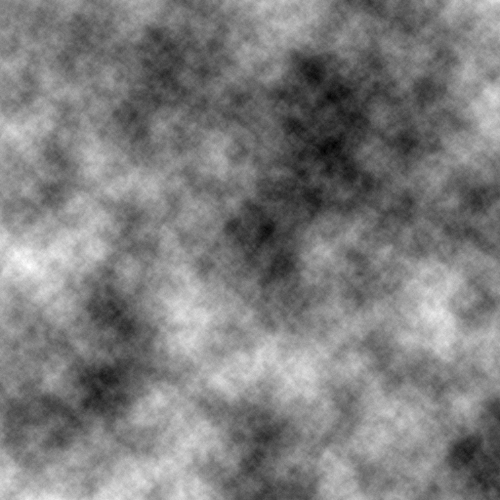
\includegraphics[width=0.45\linewidth]{fbmnoise}
    %\caption{Fbm noise}
  %\end{subfigure}
%\end{figure}

\newpage


\tsection{2. Water}


\begin{wrapfigure}{r}{0.4\textwidth}
    \centering
    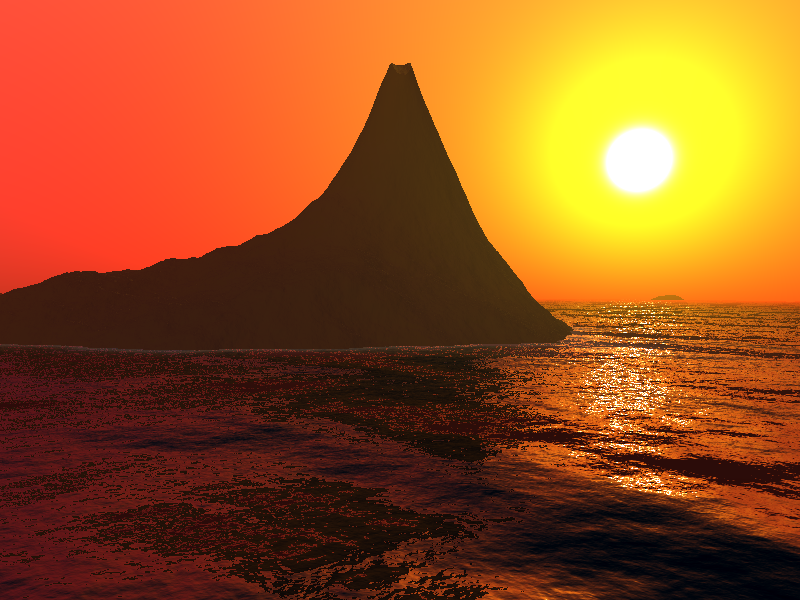
\includegraphics[width=0.38\textwidth]{water2} \par
    \caption{Very rough water reflections}
\end{wrapfigure}


The water is an important element because it breaks the boring rocky landscape into sparse small islands. 
It's not a perfect blue plane: the height of the water is modified by a sum of various semi-random \b{sine waves}, in which their argument is shifted 
proportionally with time, to simulate the flowing of the water. To the sine waves we can also add some fbm noise to give water a natural-looking roughness
on the surface:
\begin{align*}
    water\_level(x, z) =& \; y_0 + sin(x + z + time) \\
                       +& \; sin(\ldots) + \ldots + fbm(x, z)
\end{align*}
To render water reflections, the derivatives are obtained numerically, as precision was not as important.
Calling the derivatives $r_x, r_z$, the normal of the water surface  is calculated as:
\[
    n =  \Sigma_x \times \Sigma_z = (1, r_x, 0) \times (0, r_z, 1)  = (-r_x, 1, -r_z)
\]
Having the normal, calculating water reflections is very easy: just raymarch the reflected ray an adequate number of steps; if it doesn't hit anything,
render the color of the sky in that direction; otherwise, return the darker color of the terrain.

Another visually appealing effect, which is rendering the water brighter near the coasts, is achieved by:
\[
    water\_color += \frac{1}{water\_level - terrain\_level(x, z)}
\]


\tsection{3. Fog, Sun glare}
The amount of fog in a certain point at a distance $d$ from the camera is calculated with:
\[
    fog\_amount = 1 - e^{-(d^2/maxdist)}
\]
The color of the terrain is then blended with the fog color with $fog\_amount$ as the alpha amount.

To achieve a semi realistic sun glare effect, we can modify the mix the original fog color to the color of the sun (orange/yellowish) according 
to how much the camera is looking at the sun, and we calculate that with:
\[
    sun\_amount = dot(ray\_dir, sun\_dir)
\]

\begin{figure}[ht]
  \centering
  \begin{subfigure}[h]{0.5\linewidth}
    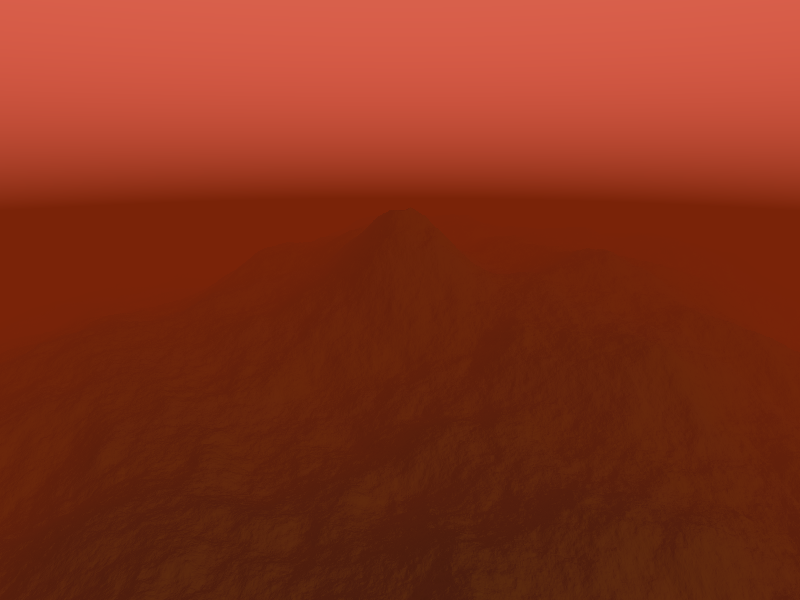
\includegraphics[width=0.95\linewidth]{fog}
    \caption{Normal fog color}
  \end{subfigure}%
  \begin{subfigure}[h]{0.5\linewidth}
    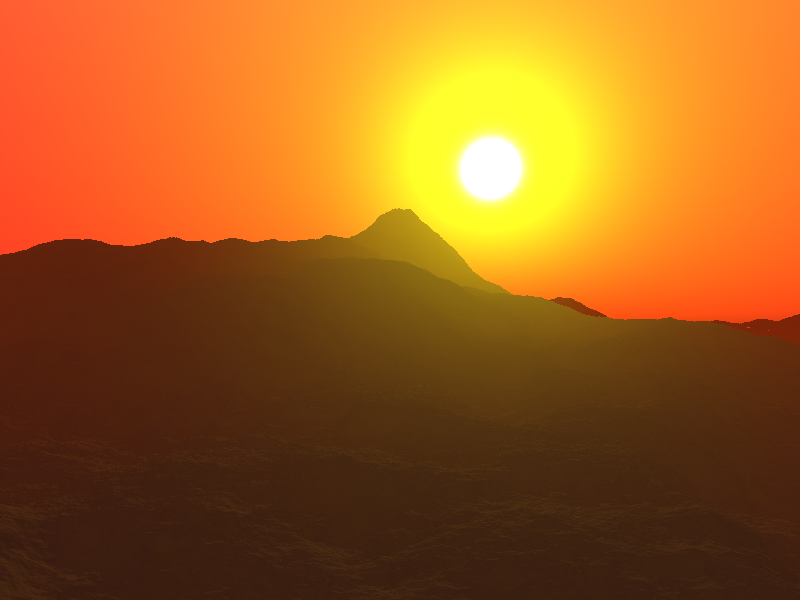
\includegraphics[width=0.95\linewidth]{fogsun}
    \caption{Fog color shifts to yellow near the sun}
  \end{subfigure}
\end{figure}


\newpage

\tsection{4. Soft shadows}
Soft shadows make lighting a lot less artificial; although usually it is very
expensive to compute soft shadows with raytracing, they are very easy to do
(and very fast) while raymarching. 

While calculating the shadow ray (the ray that goes from an object to a light source to see if it is shadowed), at each step we can get the 
penumbra (initialized at 1) this way:
\[
    penumbra = \min(penumbra, \frac{terrain(p.x, p.z) - p.y}{dist}), \quad \text{ for each step where $p$ is the raymarching position}
\]
The $penumbra$ its initialized at 1, and the lower its value is, the closer the shadow ray has passed to an obstacle between the object and the light.

\begin{figure}[ht]
  \centering
  \begin{subfigure}[h]{0.5\linewidth}
    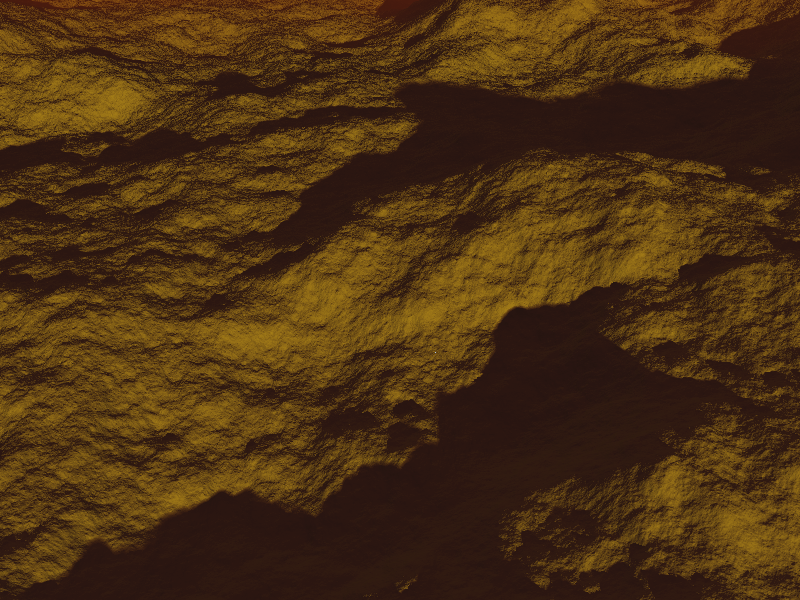
\includegraphics[width=0.95\linewidth]{hardshadows}
    \caption{Hard shadows}
  \end{subfigure}%
  \begin{subfigure}[h]{0.5\linewidth}
    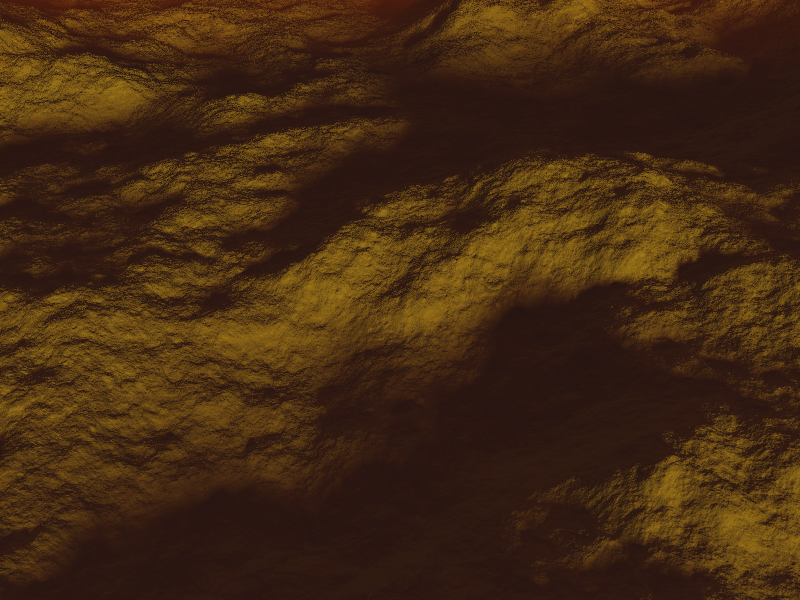
\includegraphics[width=0.95\linewidth]{softshadows}
    \caption{Soft shadows}
  \end{subfigure}
\end{figure}


\tsection{5. Special Thanks}

Inigo Quielez, for his inspiring work and his wonderful tutorials. 

Particularly useful were his \href{http://www.iquilezles.org/www/articles/fog/fog.htm}{fog tutorial}, 
and his demos \href{https://www.shadertoy.com/view/MdX3Rr}{Elevated} and \href{https://www.shadertoy.com/view/4ttSWf}{Rainforest}.

Frankenburg's \href{https://www.shadertoy.com/view/4sXGRM}{water shader} 

nimitz's \href{https://www.shadertoy.com/view/XtS3DD}{lens flare shader}

Sara Di Bartolomeo, for her amazing artistic counseling. 


\end{document}
